%%%%%%%%%%%%%%%%%%%%%%%%%%%%%%%%%%%%%%%%%
% Beamer Presentation 
% LaTeX Template
% Version 1.0 (10/11/12)
%
% This template has been downloaded from:
% http://www.LaTeXTemplates.com
%
% License:
% CC BY-NC-SA 3.0 (http://creativecommons.org/licenses/by-nc-sa/3.0/)
%
%%%%%%%%%%%%%%%%%%%%%%%%%%%%%%%%%%%%%%%%%
 
%------------------------------------------------------
%	PACKAGES
%------------------------------------------------------
\RequirePackage{currfile}
\PassOptionsToPackage{table}{xcolor}
% \documentclass[xcolor=dvipsnames]{beamer}
\documentclass[presentation]{beamer}

% Some defualt packages  
%\usepackage{CustomBeamerColor} 
\usepackage{graphicx} % Allows including images
\usepackage{booktabs} % Allows the use of \toprule, \midrule and \bottomrule in tables
\usepackage[ngerman]{babel}
\usepackage[utf8]{inputenc} 
\usepackage[T1]{fontenc} 

% bibtex:  
\usepackage[style=alphabetic,backend=biber]{biblatex}
\addbibresource{../thesis.bib}
\usepackage{csquotes}
\usepackage{silence,lmodern}
% Filter warnings issued by package biblatex starting with "Patching footnotes failed"
\WarningFilter{biblatex}{Patching footnotes failed}

%\usepackage{caption}
%\usepackage{subcaption}
\setbeamertemplate{caption}{\raggedright\insertcaption\par}

\usepackage{array}
% for notes - usage: 	\note[item]<2>{Erzähle eine Notiz!}
\usepackage{pgfpages}
%\setbeameroption{show notes} %Notizen anzeigen 
%\setbeameroption{show notes on second screen = left} 

\usepackage[table]{xcolor}    % loads also »colortbl«
\usepackage{amsmath,amssymb}
\usepackage{textpos}
\usepackage{tikz}
\setbeamertemplate{navigation symbols}{}	%remove navigation symbols
\setbeamertemplate{bibliography item}[text]
\renewcommand*{\bibfont}{\small}
%------------------------------------------------------
%	THEMES
%------------------------------------------------------
%\usetheme[]{dlr_2012}  % defines color of enumeration, background what font it is used to render whether circle or ball or rect or whatever; when you choose a presentation theme, your presentation will look the way soemone ( the creator of the theme) thought that a presentation should look like. use this theme defines everything below
\usefonttheme[]{Rosenheim}
\useinnertheme[]{Rosenheim} 	% defines how itemize environments are rendered
\useoutertheme[]{Rosenheim}	% defines where any navigational elements should go like a mini table mini frames ...and what they should look like...
\usecolortheme[]{Rosenheim} % defines the color of the outertheme

%------------------------------------------------------
%	TITLE PAGE
%------------------------------------------------------

\title[Bachelor-Thesis]{Bachelor-Thesis} % The short title appears at the bottom of every slide, the full title is only on the title page
\subtitle{Vergleich von Strategien zum dynamischen Auslagern großer 3D-Punktwolken für die schritthaltende Registrierung von Messdaten}
\author{Robert Hümmer} % Your name   
\institute[Fakultät für Informatik] % Your institution as it will appear on the bottom of every slide, may be shorthand to save space 
{
	% Your institution for the title page
	University of Applied Science Rosenheim \\
%	Institut für Robotik und Mechatronik \\
	\medskip
	\textit{robert.huemmer@gmail.com} % Your email address
}
\date{22.01.2017} % Date, can be changed to a custom date; or \today
%\titlegraphic{\includegraphics[height=10cm, keepaspectratio]{images/all_title_new.eps}}
%\titlegraphicii{\includegraphics[height=3cm, keepaspectratio]
%	{images/HS-Logo-aktuell-CMYK-eps-converted-to.pdf}}

% Outline before secion in beamer mode (usage: \OutlineAtBeginSection)
\newcommand{ 
\OutlineAtBeginSection}{
	\AtBeginSection[]
	{
		\begin{frame}{Überblick}
		\tableofcontents[currentsection]
		\end{frame}
	}
} 

%------------------------------------------------------------------------------------------

%Begriff aus dem Französischen und bedeutet Versteck. Dh. die Ersatzfunktion für das Hintergrundmedium bleibt verborgen. 
%---------------
\begin{document}
%---------------

% Maketitle (Title-Page)
\maketitle % never put this line in a frame environment

\begin{frame}
\frametitle{Umfeld}

\begin{columns}[c] % The "c" option specifies centered vertical alignment while the "t" option is used for top vertical alignment
	\column{.7\textwidth} % Left column and width
	% \textbf{Eigenschaften}
%%%%%%%%%%%%%%%%%%%%%%%
	\begin{itemize}
		\item Roboter sollen:
		\begin{itemize} 
			\item Hindernisse vermeiden
			\item Unbekannte Umgebung erkunden
			\item Objekte greifen
		\end{itemize}
		\item Wahrnehmung über Tiefenkameras
		\item Registrierung -- Anwendungsfälle:
		\begin{itemize}
		\item Lokalisation
		\item mehrere Scans zusammenführen
		\end{itemize}
		\item Lib3D-Framework (DLR-intern)
	\end{itemize}
%%%%%%%%%%%%%%%%%%%%%%%
	\column{.3\textwidth} % Right column and width
	\begin{figure}
		\centering
		\includegraphics[width=0.95\linewidth]{figures/introduction/Omnirob_dlr_version.jpg}
		\caption{omniRob \cite{Buschor2013}} 
		\label{fig:omnirob}
	\end{figure}
\end{columns} 
\end{frame} 

% Überblick 
\begin{frame}
\frametitle{Überblick}
%\pdfbookmark[2]{Überblick}{toc}
\tableofcontents
\end{frame}

%%%%%%%%%%%%%%%%%%%%%%%%%%%%%%%%%%%%%%%%%%%%%%%%%%%%%%%%%%%%%%%%%%%%%%%%%%%%%%%%%%%

\section{Motivation} 
\begin{frame}
	\frametitle{Motivation}
	\begin{itemize}
		\item Arbeitsspeicher ist teuer und begrenzt (Embedded Systemen)
		\item Vollständiges Halten der Daten im HSP nicht möglich
		\item [$\Rightarrow$] Sinnvolles Auslagern nötig
	\end{itemize}
	\begin{figure}
	\includegraphics[width=1\linewidth]{figures/introduction/registration_combined.png}
	\caption{Beispiele großer Punktwolken (aus \cite{PCLReg})}
	\end{figure} 
\end{frame}

\section{Lösungsansätze}
\begin{frame}
	\frametitle{Lösungsansätze}
	\begin{figure} 
		\centering
		\begin{minipage}{.5\textwidth}
			\centering
			\includegraphics[width=0.90\linewidth]{figures/introduction/mot1.png}
			\caption{(a) Auslagern alles hinter der Kamera liegend}
			\label{fig:sub1}
		\end{minipage}%
		\begin{minipage}{.5\textwidth} 
			\centering
			\includegraphics[width=0.90\linewidth]{figures/introduction/mot2.png}
			\caption{(b) Auslagern alles außerhalb eines bestimmten Radius}
			\label{fig:sub2}
		\end{minipage}
	\label{fig:test} 
\end{figure}
\end{frame}

\begin{frame}
\frametitle{Lösungsansätze} 
\color{dd-gray} \textbf{Einsatz von } \color{black} 
\begin{itemize}
	\item Caching-Strategien % Führen Statistik über Zugriffe/Zugriffsmuster
\end{itemize}

\color{dd-gray} \textbf{Anforderungen} \color{black} 
\begin{itemize}
\item Eine gute Cache-Hit-Rate erzielen
\item Laufzeit- sowie Speichereffizient (wenig Overhead)
\end{itemize}
\end{frame}

\section{Ziel der Arbeit}
\begin{frame}
	\frametitle{Ziel der Arbeit} % + Was ist überhaupt ein Cache + Metrik um Caches zu vergleichen
	\color{dd-gray} \textbf{Ziel:} \color{black} 
	\begin{itemize}
	\item Sinnvolles und effizientes Auslagern mithilfe bereits existierender Caching-Strategien
	\end{itemize}
	
	\color{dd-gray} \textbf{Dazu ist nötig:} \color{black} 
	\begin{itemize} 
	\item Einbringen der Strategien in den Registrierungs-Prozess \\ (Lib3D-Framework)  % Wo das Caching anzubringen ist?
	\item Entscheidung was genau auszulagern ist \\ (siehe Extendable Octree)
	\end{itemize}
\end{frame}

%%%%%%%%%%%%%%%%%%%%%%%%%%%%%%%%%%%%%%%%%%%%%%%%%%%%%%%%%%%%%%%%%%%%%%%%%%%%%%%%%%%

\section{Caching-Strategien}

\begin{frame}
\frametitle{Caching-Strategien}
\begin{itemize}
	\item Vermeidung einer Strategie, die eine offline Auswahl eines optimierbaren Parameters benötigt
\end{itemize}
\end{frame}


\begin{frame}
\frametitle{Least Recently Used (LRU)}
Verdrängt das Element, auf das in der Vergangenheit am seltensten zugegriffen wurde. \\
\vspace{0.3cm}
% Basiert auf zeitlicher Lokalität

%\note{ 
%	Nutzt die zeitliche 
%	limitiert sich selbst nur an der Information der Zeit der Referenz... (zu wenig Infos die es verwendet)
%	Ist nicht in der Lage zwischen Elementen mit regelmäßigen Zugriffen und unregelmäßigen Zugriffen zu unterscheiden... Je nach Datensatz => verschwendeter Speicherplatz mit Elementen mit unregelmäßigen Zugriff...
%	
%	Zu wenig infos: Einfach die Zeit des letzten Zugriffs implizit gespeichert durch die Position im einer Queue 
%	Basiert auf zeitliche Lokalität. Dh. Sehr gut für zeitlich geclusterte Zugriffsmuster.
%}  
\vspace{0.3cm}
%\pause
\color{dd-gray} \textbf{Vorteile} \color{black} 
\begin{itemize}%[<+->]
	\item Einfache Implementierung -- nur eine Information nötig % (die Aktualität)
	\item wenig Speicher-Overhead
\end{itemize}

%\pause
\color{dd-gray} \textbf{Nachteile} \color{black} 
\begin{itemize}%[<+->]
	\item Bezieht keine Zugriffs-Häufigkeiten mit ein
\end{itemize}
\end{frame}

\begin{frame}
\frametitle{Adaptive Replacement Cache (ARC)}

\color{dd-gray} \textbf{Datenstruktur:} \color{black} 
\begin{figure}
\includegraphics[width=0.9\linewidth]{figures/caches/arc} 
\caption{Schema der Datenstruktur von ARC (basierend auf \cite{megiddo2003arc})}
\end{figure} 
%\color{dd-gray} \textbf{Eigenschaften:} \color{black} 
%\begin{itemize}
%\item Scan-Resistant % durch die einteilung in 2 Listen Ähnlich wie bei SLRU
%\item Low-Overhead
%\item Adaptiv (selbstlernend) % Vorteil: keine zusätzlichen Parameter
%%\note{Lernt über fälschlicherweise verdrängte Elemente mit einer Regret-Value} % vergleicht bei einem Cache Miss die Wahrscheinlichkeiten eines Hits in B1 zu einem Hit in B2  
%% \item Ghost Entries -- Einträge von bereits verdrängte Elemente
%%	\item Häufig: neues Element wird dem Cache immer hinzugefügt und der Cache kümmert sich einzig und allein um die Verdrängungsstrategie eines Elements
%%-> Grund: Das managen von meta-daten für Elemente die sich gerade nicht im Cache befinden wäre nicht praktisch...
%\end{itemize}
\end{frame}

%%%%%%%%%%%%%%%%%%%%%%%%%%%%%%%%%%%%%%%%%%%%%%%%%%%%%%%%%%%%%%%%%%%%%%%%%%%%%%%%%%%

\OutlineAtBeginSection
\section{Analyse}  % oder \section{Analyse der Architektur}

% \subsection{Prozess ohne Caching}
\begin{frame}
\frametitle{Prozess ohne Caching}
\begin{figure}
	\centering
	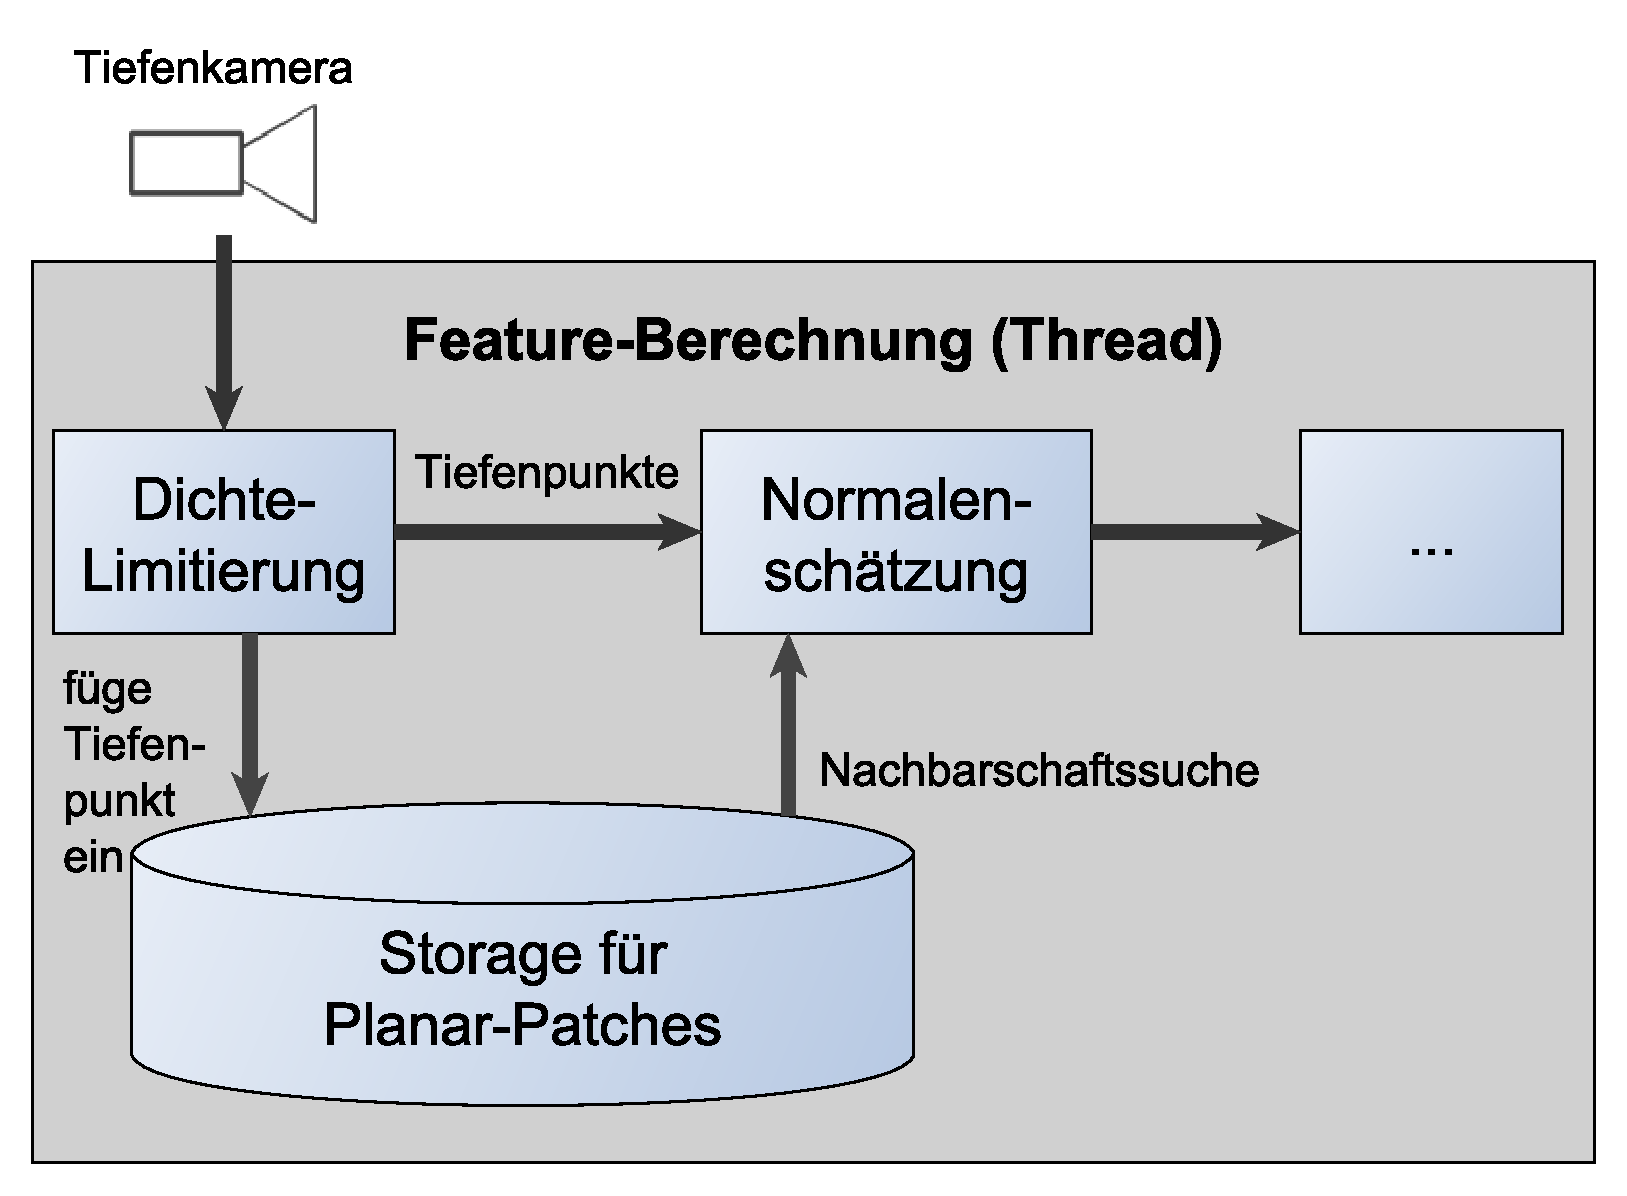
\includegraphics[width=0.7\linewidth]{figures/relatedWorks/FeatureEstimationProcessSimplified.pdf}
	\caption{Teil des streambasierten Prozesses der Feature-Berechnung}
	\label{fig:sub3} 
\end{figure}

%Es gibt noch weitere Prozessierungsschritte, die hier nicht abgebildet sind (für mehr Informationen hierzu siehe Bachelorarbeit)

\end{frame}

%--- Datenstruktur (Extendable Octree)

\begin{frame}
\frametitle{Extendable Octree}
\begin{itemize}%[<+->]
	\item Punkte werden in den Leaf-Nodes (Voxel) des Extendable Octrees abgelegt 
\end{itemize}
\begin{figure}
\centering
\includegraphics[width=0.3\linewidth]{figures/relatedWorks/voxel_definition.png}
\caption{Definition eines Voxels (Abbildung aus \cite{Bodenmueller2009})}
\label{fig:voxel}
\end{figure}
%\begin{columns}[c] % The "c" option specifies centered vertical alignment while the "t" option is used for top vertical alignment
%	\column{.3\textwidth} % Left column and width
%	% \textbf{Eigenschaften}
%	%%%%%%%%%%%%%%%%%%%%%%%
%	\begin{figure}
%		\centering
%		\includegraphics[width=0.6\linewidth]{figures/voxel_definition.png}
%		\caption{Definition eines Voxels (Abbildung aus \cite{Bodenmueller2009})}
%		\label{fig:voxel}
%	\end{figure}
%	%%%%%%%%%%%%%%%%%%%%%%%
%	\column{.7\textwidth} % Right column and width
%	\begin{figure}
%		\centering
%		\includegraphics[width=1\linewidth]{figures/ExtendableOctreeConstruction.png}
%		\caption{Aufbau des Extendable Octrees (Abbildungen aus \cite{Bodenmueller2009})}
%		\label{fig:ExtendableOctree}
%	\end{figure}
%\end{columns} 
\end{frame}

\begin{frame}
\frametitle{Analyse des Speicherbedarfs}
\begin{figure}
\centering
\includegraphics[width=0.7\linewidth]{figures/Benchmark_withoutCaching.png}
\caption{Speicherbedarf des Extendable Octree (ohne Caching)} %: Reduktionsradius von $r_r$ von 0 (Dichte-Limitierung) und einer Voxel-Auflösung von $1$ statt.
\label{fig:BenchmarkWithoutCaching} 
\end{figure} 
\end{frame} 

%%%%%%%%%%%%%%%%%%%%%%%%%%%%%%%%%%%%%%%%%%%%%%%%%%%%%%%%%%%%%%%%%%%%%%%%%%%%%%%%%%%

\OutlineAtBeginSection
\section{Konzepte}

% \subsection{Prozess mit Caching}
\begin{frame}
\frametitle{Prozess mit Caching}
\begin{figure}
	\centering
	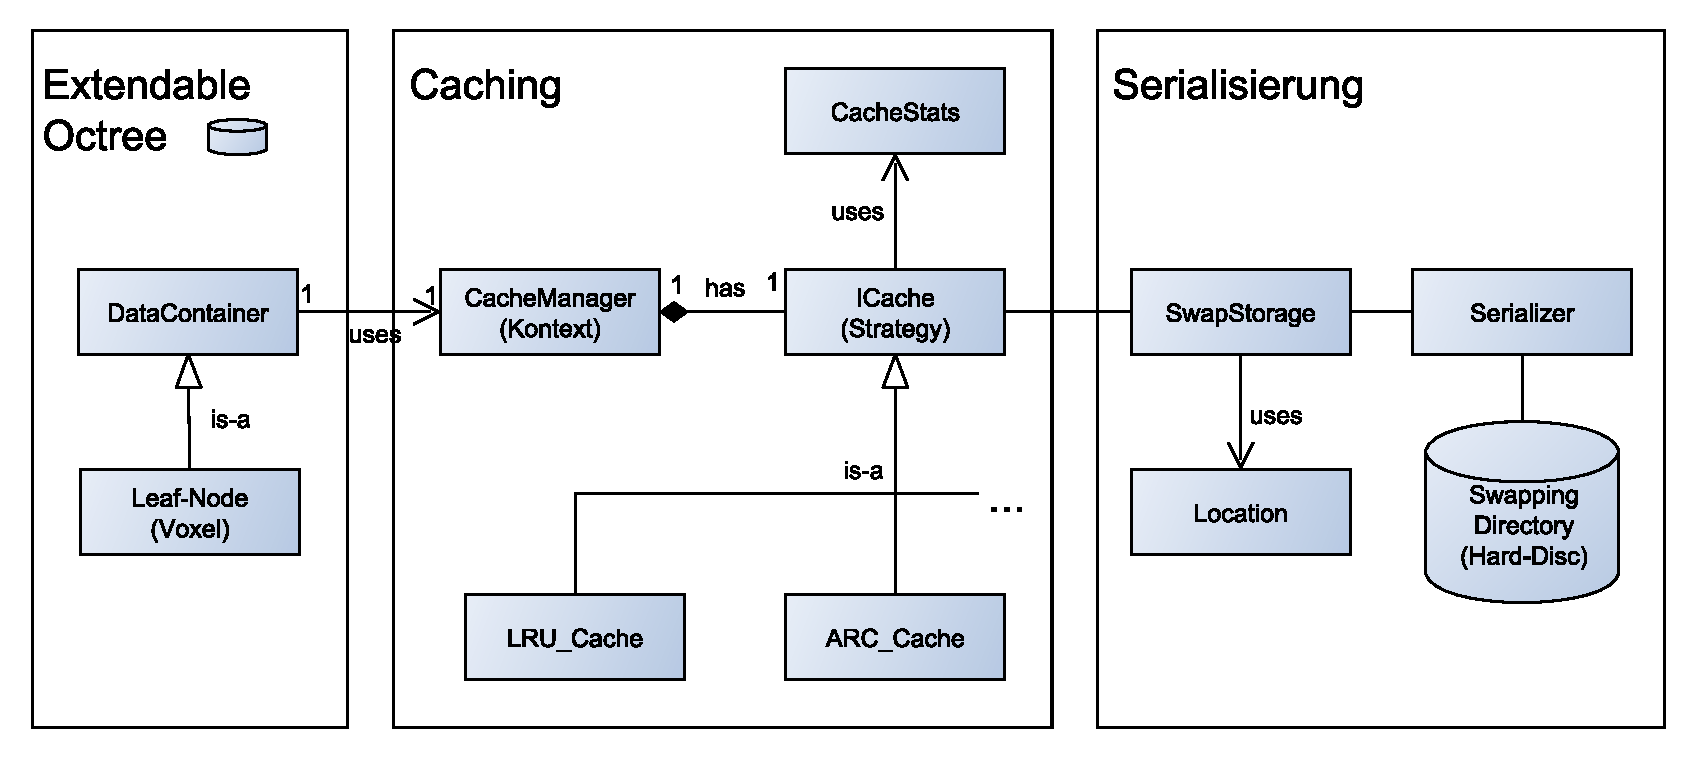
\includegraphics[width=1\linewidth]{figures/concepts/CacheConcept2.pdf}
	\caption{Erweiterung der Feature-Berechnung (Feature-Estimation)}
	\label{fig:sub4}
\end{figure}
\end{frame}

\begin{frame}
\frametitle{Problematik dynamischer Elemente} 

\begin{itemize}
	\item Existierende Caching-Strategien basieren auf Elemente fester Größe
	\item In dieser Anwendung sind die gecachten Elemente jedoch Voxelinhalte, die sich dynamisch in ihrer Größe verändern
\end{itemize}
\end{frame} 


% \subsection{Update-Konzept}
\begin{frame}
\frametitle{Update-Konzept} 
\begin{figure}
\centering
\includegraphics[width=0.40\linewidth]{figures/concepts/mutableCachedEntriesConcept.png}
\caption{Schema zum Benachrichtigen des Caches bei Größenänderung}
\label{fig:sub5}
\end{figure}
\begin{itemize}
	\item STD: Pro Container-Typ ein zustandsloser Allokator
	\item EASTL: Pro Container-Instanz ein Allokator
\end{itemize}
\end{frame}

%%%%%%%%%%%%%%%%%%%%%%%%%%%%%%%%%%%%%%%%%%%%%%%%%%%%%%%%%%%%%%%%%%%%%%%%%%%%%%%%%%%

\OutlineAtBeginSection
\section{Ergebnisse}
\begin{frame}
	\frametitle{Ergebnisse}
	\vskip0.25\baselineskip
	\color{dd-gray} \textbf{Vergleich der Hit-Rate} \color{black}

	\begin{columns}[c] % The "c" option specifies centered vertical alignment while the "t" option is used for top vertical alignment
		\column{.4\textwidth} % Left column and width
		% \textbf{Eigenschaften}
		\begin{figure}
			\centering
			\includegraphics[width=1\linewidth]{figures/Unikirche2.png}
			\caption{Illustration des Datensatzes \emph{Unikirche} (3D-Punktwolke)}
			\label{fig:sub6}
		\end{figure}
		\column{.6\textwidth} % Right column and width
		\begin{figure}
			\centering
			\includegraphics[width=0.9\linewidth]{figures/results/DensityLimitationHitRates.png}
			\caption{Zeigt, dass die Cache-Hit-Rate von LRU besser ist als die von ARC}
			\label{fig:sub7}
		\end{figure}
	\end{columns}
%	\begin{itemize}
%	\space
%	\item Grund für die gute Cache-Hit-Rate:
%		\begin{itemize}\space
%			\item[$\rightarrow$] Große Anzahl an einzufügenden Punkten in die Voxel
%			\item[$\Rightarrow$] Voxel werden entsprechend häufig angefragt
%		\end{itemize}
%	\end{itemize} 
\end{frame}

 
\begin{frame}
\frametitle{Ergebnisse}
\vskip0.25\baselineskip
\color{dd-gray} \textbf{Vergleich der Swapping-Kosten} \color{black}
\begin{columns}[c] % The "c" option specifies centered vertical alignment while the "t" option is used for top vertical alignment
	\column{.5\textwidth} % Left column and width
	% \textbf{Eigenschaften}
	\begin{figure}
		\centering
		\includegraphics[width=1\linewidth]{figures/results/DensityLimitationSwapUnloadCosts.png}
		\caption{}
		\label{fig:sub8}
	\end{figure}
	\column{.5\textwidth} % Right column and width
	\begin{figure}
	\centering
	\includegraphics[width=1\linewidth]{figures/results/DensityLimitationSwapLoadCosts.png}
	\caption{}
	\label{fig:sub9}
	\end{figure}
\end{columns}
% note: was die laufzeit betrifft so sind inserts und gets konstanter laufzeit
% kein rumkopieren, keine prioritätswarteschlane, Referenzen werden umgehängt und Hash-Tabelle als schneller Lookup, um die Position des gecachten Elements über den jeweiligen Iterator zu finden.
\end{frame} 

\OutlineAtBeginSection
\section{Zusammenfassung und Ausblick}
\begin{frame}
	\frametitle{Zusammenfassung}
	%%%inhaltlich Folien so zusammenstellen, dass hier mindestens 3 Punkte stehen...
	\begin{itemize}
		\item Auslagern der Voxelinhalte des Extendable Octrees\\(pro Voxelinhalt eine Binärdatei)
		\item Identifikation der Voxelinhalte über die Speicheradresse des Leaf-Nodes
		\item Update-Konzept zur Rückmeldung über den von Voxelinhalten angelegten Speicher
		\item ARC hat sich als schlechter herausgestellt
		\item Aufeinanderfolgende Zugriffe auf Voxelinhalte bei der Dichte-Limitierung sowie Feature-Berechnung sind räumlich und zeitlich nah beieinander
	\end{itemize} 
\end{frame}
 
 
% HDF-Format, LIRS, Threading beim Auslagern 
\begin{frame}
	\frametitle{Ausblick}
	\begin{itemize}
		\item Verwendung des Dateiformats \emph{Hierarchical Data Format} (HDF)
		%\item Locking von gecachten Elementen (Lock-Bits)
		\item LIRS können noch untersucht werden (Metrik: IRR) % evtl sogar besser als LRU; update konzept hier sogar hilfreich!
		%\item Einsatz von GDSF, um die Swapping-Kosten gering zu halten
	\end{itemize}
\end{frame}

%------------------------------------------------------------------------------------------
% following cites to be included in the bibliography:
\nocite{podlipnig2003survey}
\nocite{karedla1994caching}
\nocite{cherkasova1998improving} 
%------------------------------------------------------------------------------------------

\begin{frame}  % allowframebreaks
	%\AtBeginBibliography{\small}
	\frametitle{Referenzen}
	\printbibliography[heading=none]
\end{frame}
 
% \subsection{Testdaten}
\begin{frame}
\frametitle{Ergebnisse}
\vskip0.25\baselineskip
\color{dd-gray} \textbf{Testdaten} \color{black}

% Annahme wenn die Dichte-Limitierung mit Caching bei diesen Datensatz gut ausfällt, dann ist auch die Feature-Berechnung gut. Zugriffsmuster ändert sich bei der Registrierung kaum. Lediglich kommt noch eine Berechnung der Nachbarschaft hinzu dadurch wird jedoch das Zugriffsmuster nicht sonderlich beeinflusst. 

\begin{itemize}
	\item Punktwolke einer Unikirche
	\item Voxel-Auflösung von $0.01$
	\item Dichte-Limitationsradius von $0.000561231$ 
\end{itemize}

\begin{figure}
	\centering
	\includegraphics[width=0.55\linewidth]{figures/Unikirche2.png}
	\caption{Illustration des Datensatzes \emph{Unikirche}}
	\label{fig:sub11}
\end{figure}
\end{frame}

\begin{frame}
\frametitle{Ergebnisse}
\vskip0.25\baselineskip
\color{dd-gray} \textbf{Vergleich der Hit-Rate} \color{black}

\begin{columns}[c] % The "c" option specifies centered vertical alignment while the "t" option is used for top vertical alignment
	\column{.4\textwidth} % Left column and width
	% \textbf{Eigenschaften}
	\begin{itemize}\space
		\item Cache-Inserts (ohne unload):  \\ $69.475$ (entspricht gesamte Voxelanzahl)
		\item Cache-Gets: \\\space$11.663.094$ 
		\item[$\Rightarrow$] Gets pro Voxelinhalt durchschnittlich $\approx 168$
	\end{itemize}
	\column{.6\textwidth} % Right column and width
	\begin{figure}
		\centering
		\includegraphics[width=0.9\linewidth]{figures/results/DensityLimitationHitRates.png}
		\caption{Zeigt, dass die Cache-Hit-Rate von LRU besser ist als die von ARC}
		\label{fig:sub12}
	\end{figure}
\end{columns}
%	\begin{itemize}
%	\space
%	\item Grund für die gute Cache-Hit-Rate:
%		\begin{itemize}\space
%			\item[$\rightarrow$] Große Anzahl an einzufügenden Punkten in die Voxel
%			\item[$\Rightarrow$] Voxel werden entsprechend häufig angefragt
%		\end{itemize}
%	\end{itemize} 
\end{frame}

\begin{frame}
\frametitle{Problematik ungültiger Referenzen}
%\vskip0.25\baselineskip
%\color{dd-gray} \textbf{Problematik ungültiger Referenzen} \color{black}

% Annahme wenn die Dichte-Limitierung mit Caching bei diesen Datensatz gut ausfällt, dann ist auch die Feature-Berechnung gut. Zugriffsmuster ändert sich bei der Registrierung kaum. Lediglich kommt noch eine Berechnung der Nachbarschaft hinzu dadurch wird jedoch das Zugriffsmuster nicht sonderlich beeinflusst. 

\begin{figure}
	\centering
	\includegraphics[width=0.8\linewidth]{figures/problematikDerLookupTable.png}
	\caption{Zeigt die Problematik ungültiger Referenzen}
	\label{fig:su13}
\end{figure}
\end{frame}


%-------------
\end{document}
%-------------
